% !TeX root = ../../navier-stokes-manuscript.tex
\begin{figure}[!htbp]
  \centering
  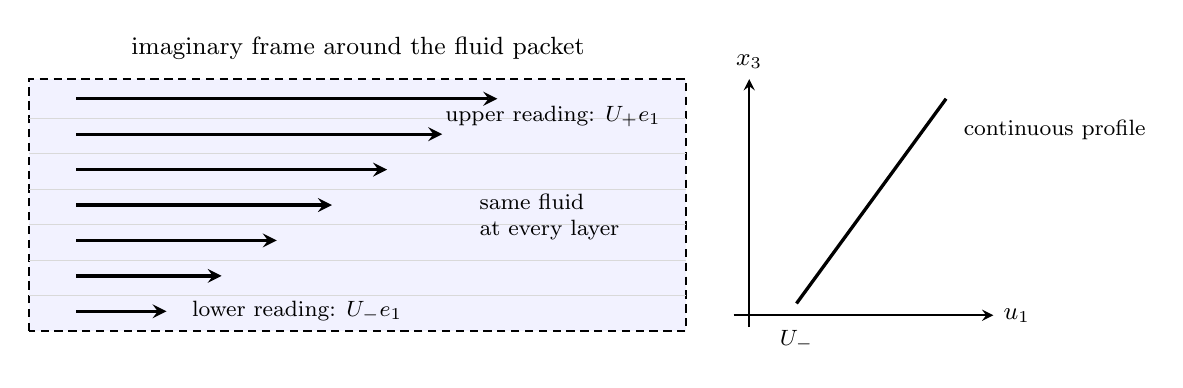
\begin{tikzpicture}[
    x=1cm,
    y=1cm,
    >=stealth,
    velocity/.style={->,very thick},
    smalllabel/.style={font=\small},
    tinylabel/.style={font=\footnotesize}
  ]
    \fill[blue!5]
      (0.50,0.65) rectangle (8.85,3.85);
    \draw[densely dashed,thick]
      (0.50,0.65) rectangle (8.85,3.85);

    \foreach \y in {1.10,1.55,2.00,2.45,2.90,3.35}
      \draw[black!15] (0.50,\y) -- (8.85,\y);

    \draw[velocity] (1.10,0.90) -- (2.25,0.90);
    \draw[velocity] (1.10,1.35) -- (2.95,1.35);
    \draw[velocity] (1.10,1.80) -- (3.65,1.80);
    \draw[velocity] (1.10,2.25) -- (4.35,2.25);
    \draw[velocity] (1.10,2.70) -- (5.05,2.70);
    \draw[velocity] (1.10,3.15) -- (5.75,3.15);
    \draw[velocity] (1.10,3.60) -- (6.45,3.60);

    \node[tinylabel,anchor=east] at (8.65,3.38)
      {upper reading: \(U_+e_1\)};
    \node[tinylabel,anchor=west] at (2.45,0.90)
      {lower reading: \(U_-e_1\)};
    \node[smalllabel,anchor=south] at (4.68,3.98)
      {imaginary frame around the fluid packet};
    \node[tinylabel,align=left,anchor=west] at (6.10,2.10)
      {same fluid\\at every layer};

    \draw[->,thick] (9.65,0.70) -- (9.65,3.85)
      node[above,smalllabel] {\(x_3\)};
    \draw[->,thick] (9.45,0.85) -- (12.75,0.85)
      node[right,smalllabel] {\(u_1\)};
    \draw[very thick] (10.25,1.00) -- (12.15,3.60);
    \node[tinylabel,anchor=north] at (10.25,0.78) {\(U_-\)};
    \node[tinylabel,anchor=west] at (12.25,3.20)
      {continuous profile};
  \end{tikzpicture}
  \caption{Continuous shear imagined inside one fluid packet.
  The dashed outline is only an observation frame.
  Every layer takes an intermediate velocity, so the one velocity field remains smooth across the packet.}
  \label{fig:CouetteFlow}
\end{figure}
